\documentclass{beamer}

% Español
%\usepackage[spanish]{babel}
\usepackage[utf8]{inputenc}
\usepackage[T1]{fontenc}

% Tipo de letra
\usepackage{palatino}

% Plantilla
\usetheme{Antibes}
%\usetheme{Berlin}


%\usepackage[scale=1.2]{ccicons}

\usepackage{listings}
\lstdefinestyle{cpp11}{
  belowcaptionskip=1\baselineskip,
  breaklines=true,
  xleftmargin=\parindent,
  language=C++,
  showstringspaces=false,
  basicstyle=\scriptsize\ttfamily,
  keywordstyle=\bfseries\color{green!40!black},
  commentstyle=\itshape\color{purple!40!black},
  identifierstyle=\color{blue},
  stringstyle=\color{orange},
  columns=flexible,
  %inputenconding=utf8,
  extendedchars=true,
  morekeywords=[1]{_Pragma,constexpr,nullptr,alignof,alignas},
  literate=%
    {¿}{{?`}}1
    {á}{{\'a}}1
    {é}{{\'e}}1
    {í}{{\'i}}1
    {ó}{{\'o}}1
    {ú}{{\'u}}1
    {ñ}{{\~n}}1
}

\newcommand{\cppkey}[1]{%
{\color{green!40!black}\textbf{\texttt{#1}}}%
}

\newcommand{\cppid}[1]{%
{\color{blue}\texttt{#1}}%
}

\setbeamertemplate{footline}{
  \leavevmode%
  \hbox{\begin{beamercolorbox}[wd=\paperwidth,ht=2.5ex,dp=1.125ex,leftskip=.3cm,rightskip=.3cm]{author in head/foot}%
    \usebeamerfont{author in head/foot} J. Daniel Garcia -- ARCOS@UC3M (josedaniel.garcia@uc3m.es)
    \hfill
    \insertframenumber/\inserttotalframenumber
  \end{beamercolorbox}}%
  \vskip0pt%
}

\usepackage{tikz}
\usetikzlibrary{positioning}
\usetikzlibrary{arrows}
\usetikzlibrary{mindmap}

\usepackage{pgfplots}
\pgfplotsset{compat=1.5}

\usepackage{tabularx}

\addtobeamertemplate{headline}{}
{% 
\begin{tikzpicture}[remember picture,overlay]
\node[anchor=north east] at (current page.north east) {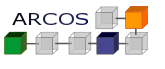
\includegraphics[height=0.7cm]{logos/arcos.png}};
\end{tikzpicture}
}


  \tikzset{
    invisible/.style={opacity=0},
    visible on/.style={alt=#1{}{invisible}},
    alt/.code args={<#1>#2#3}{%
      \alt<#1>{\pgfkeysalso{#2}}{\pgfkeysalso{#3}} % \pgfkeysalso doesn't change the path
    },
  }

%Portada
\title{Run-time bound array data members}
\author{J. Daniel Garcia and Xin Li}
\institute{Universidad Carlos III de Madrid}
\date{\today}

\begin{document}

\begin{frame}
\titlepage
\end{frame}

\AtBeginSection[]
{
  \begin{frame}<*>
    \setbeamertemplate{section in toc shaded}[default][50]
    \setbeamertemplate{subsection in toc shaded}[default][50]
    \tableofcontents[currentsection,hideallsubsections]
  \end{frame}
}

\AtBeginSubsection[]
{
  \begin{frame}<beamer>
    \setbeamertemplate{subsection in toc shaded}[default][50]
    \tableofcontents[sectionstyle=show/hide,subsectionstyle=show/shaded/hide]
  \end{frame}
}

\begin{frame}{Thanks to}
\begin{itemize}
  \item This proposal is heavily based on N3810 (B. Stroustrup).
  \item This proposal incorporates ideas from discusions with Daveed Vandevoorde, Bjarne Stroustrup, and Lawrence Crowl.
  \item A partial prototype implementation of some ideas have been done on gcc by Xin Li.
\end{itemize}
\end{frame}

\section{Problem}

\begin{frame}{The problem with VLA's}
  \begin{itemize}
    \item Variable Length Arrays in C since C99.
      \begin{itemize}
        \item Problematic in C++.
      \end{itemize}
    \item Past proposals:
      \begin{itemize}
        \item Runtime-sized arrays with automatic storage.
          \begin{itemize}
            \item N3366, N3412, N3467, N3497, N3639.
          \end{itemize}
        \item \texttt{dynarray}.
          \begin{itemize}
            \item N3532, N3662
          \end{itemize}
        \item \texttt{bs\_array}.
          \begin{itemize}
            \item N3810
          \end{itemize}
      \end{itemize}
    \item Alternatives sumarized in N3810.
  \end{itemize}
\end{frame}

\subsection{Runtime-sized arrays with automatic storage}

\begin{frame}[fragile]{Use case}
  \begin{itemize}
    \item A user wishes to allocate a local array whose size is not known at compile-time, but at runtime only.
  \end{itemize}
\pause
\begin{lstlisting}[style=cpp11]
std::string f(int n) {
  std::vector<int> v(n); // std::vector allocation
  std::iota(v.begin(), v.end(), 1);
  std::string result;
  for (auto x : v) {
    result += std::to_string(x);
  }
  return result;
} // std::vector deallocation
\end{lstlisting}
  \begin{itemize}
    \item \alert{Use of memory allocation leads to performance penalty}.
  \end{itemize}
\end{frame}

\begin{frame}[t,fragile]{Avoiding dynamic memory allocation}
  \begin{itemize}
    \item \emph{Use a runtime sized array with automatic storage}.
  \end{itemize}
\begin{lstlisting}[style=cpp11]
std::string f(int n) {
  int v[n]; // run-time sized array with automatic storage
  std::iota(v, v + n, 1);
  std::string result;
  for (int i=0; i<n; ++i) {
    result += std::to_string(x);
  }
  return result;
} 
\end{lstlisting}
\end{frame}

\begin{frame}[t,fragile]{Promoting pointer-plus-size interface}
\begin{lstlisting}[style=cpp11]
std::string g(int * v, std::size_t n) {
  std::string result;
  for (std::size_t i=0; i!=n; ++i) {
    result += std::to_string(v[i]);
  }
  return result;
}

std::string f(int n) {
  int v[n];
  std::iota(v, v + n, 1);
  return g(v, n);
} 
\end{lstlisting}
\pause
\begin{itemize}
  \item Why this interface is not desirable?
    \begin{itemize}
      \item Number of elements not available $\Rightarrow$ User needs to \emph{remember} size.
      \item Type to access elements can implicitly changes after array decayed to pointer.
    \end{itemize}
\end{itemize}
\end{frame}

\subsection{\texttt{dynarray} class}

\begin{frame}{\texttt{dynarray}}
  \begin{itemize}
    \item A class with compiler support to eventually allocate on stack.
      \begin{itemize}
        \item A pure-library implementation is possible.
        \item But it would probably be based on dynamic memory allocation.
        \item Stack allocation would require \emph{compiler magic}.
      \end{itemize}
    \item Pro:
      \begin{itemize}
        \item It solves the \emph{interface problem}.
      \end{itemize}
    \item Con:
      \begin{itemize}
        \item \texttt{dynarray} evolved to \emph{almost a container}.
        \item No guarantee whether an object will be allocated in automatic or dynamic storage.
      \end{itemize}
  \end{itemize}
\end{frame}

\begin{frame}[t,fragile]{Using \texttt{dynarray}}
\begin{lstlisting}[style=cpp11]
std::string g(const dynarray<int> & v) {
  std::string result;
  for (auto x : v) {
    result += std::to_string(x);
  }
  return result;
}

std::string f(int n) {
  dynarray<int> v{n}; // Where is this allocated?
  std::iota(v.begin(), v.end(), 1);
  return g(v);
} 
\end{lstlisting}
\end{frame}

\subsection{\texttt{bs\_array} class}

\begin{frame}[t,fragile]{A \emph{minimal stack-allocated array}}
\begin{lstlisting}[style=cpp11]
template<class T>
class bs_array { // basic stack-allocated array
public:
  using value_type = T;

  bs_array(int n); // n elements
  T& operator[](int i); 
  const T& operator(int i) const; 
  T& at(int i); 
  const T& at(int i) const; 
  T* begin() { return a; } 
  const T* begin() const { return a; }
  T* end() { return a+n; }
  const T* end() const { return a+n; }
  int size();
  T* data();
private:
  T a[n]; // for exposition only, a is stack allocated
};
\end{lstlisting}
\end{frame}

\begin{frame}[t,fragile]{Using \texttt{bs\_array}}
\begin{lstlisting}[style=cpp11]
std::string g(const bs_array<int> & v) {
  std::string result;
  for (auto x : v) {
    result += std::to_string(x);
  }
  return result;
}

std::string f(int n) {
  bs_array<int> v{n}; // allocated on the stack
  std::iota(v.begin(), v.end(), 1);
  return g(v);
}
\end{lstlisting}
\begin{itemize}
  \item It always allocates on the stack.
  \item No wrong interface promotion.
  \item \alert{Needs compiler support}.
\end{itemize}
\end{frame}

\section{Minimal proposal}

This paper introduces a minimal proposal with a strawman syntax for it.
Thus, syntax here is used only for illustration. Besides, additional
features could be elaborated if there is some agreement on the notions
presented in this paper.

\subsection{Design principles}

This proposal follows the guidance quoted in the introduction of this paper.
Moreover the design of this proposal tries to follow a set of design principles:

\begin{enumerate}
\item An operation contract should allow to express its preconditions and its
postconditions as part of its declaration.
\item The language should offer tools for expressing invariants at different
scopes.
\item Violation of a contract should be handled orthogonally from run-time
errors due to abnormal conditions.
\item Contracts should be well integrated with polymorphism.
\end{enumerate}



\end{document}
